%==================================================================%
% Author : Tezanos Iba�ez, Angel                                   %
%          S�nchez Barreiro, Pablo                                 %
% Version: 1.0, 02/03/2011                                         %
%                                                                  %
% Memoria del Proyecto Fin de Carrera                              %
%==================================================================%

\documentclass[a4paper,11pt]{itsas_pfc}

%=====================================================================%
%                       My imported packages                          %
%=====================================================================%
\usepackage[latin1]{inputenc}
\usepackage{longtable}
\usepackage{array}
\usepackage{url}
\usepackage{amsfonts}
\usepackage[spanish,activeacute]{babel}

% Esto se a�ade porque a alg�n gracioso le apetec�a que la fuente
% de la portada fuese Arial
\usepackage[T1]{fontenc}
\usepackage[scaled]{uarial}


% File with main configuration
%
% Potentially useful packages (rec = recommended, opt = optional)
%
\usepackage{fancyhdr}          % (rec)  allows for the customization of various header/footer parameters
% \usepackage{courier}         % (opt)  uses that font by default
% \usepackage{setspace}        % (opt)  allows for inter-line space changing
\usepackage{longtable}         % (opt)  allows for multi-page tables
% \usepackage{lscape}          % (opt)  allows for the use of \landscape
\usepackage{color}             % (opt)  various color-related commands (like \color)
\usepackage{rotating}          % (opt)  allows for PS and EPS rotation
% \usepackage{textcomp}        % (opt)  allows for euro sign, with \texteuro
\usepackage[spanish]{minitoc}           % (opt)  allows for per-chapter tables of contents
\usepackage{epsf}              % (opt)  allow for certain EPS manipulations
%\usepackage[utf8x]{inputenc}  % (opt)  allows for some text editors to show \'{a} as �, and so on.
\usepackage[absolute]{textpos} % (rec)  allows for arbitrary positioning of text (required for default cover page)
% \usepackage{srcltx}            % (opt)  allows to pass from .dvi back to the .tex
%
% Margin settings. Uncomment and modify if you know what you are doing. Note
% that a further 1 inch is added to the margins given here. The given values are
% the default ones for A4 paper, and itsas_pfc.cls style.
%
\setlength{\oddsidemargin}{0.3in}     % left margin for odd (right) pages
\setlength{\evensidemargin}{0.3in}    % left margin for even (left) pages
\setlength{\textwidth}{6in}        % width of the text body


%
% Recommended to improve the automatic positioning of figures.
% (taken from http://dcwww.camp.dtu.dk/~schiotz/comp/LatexTips/LatexTips.html#captfont)
%
\renewcommand{\topfraction}{0.85}
\renewcommand{\textfraction}{0.1}
\renewcommand{\floatpagefraction}{0.75}

%
% Space between top border of page and where text begins (headers go there)
% LaTeX complains if using package fancyhdr and headheight is below 15pt
%
\headheight 15pt

%
% For the textpos package (used when making the cover page)
%
\setlength{\TPHorizModule}{\paperwidth}
\setlength{\TPVertModule}{\paperheight}
\newcommand{\tb}[4]{\begin{textblock}{#1}[0.5,0.5](#2,#3)\begin{center}#4\end{center}\end{textblock}}

%
% You can define your commands here
%
% \newcommand{cmd}[args]{def}
% cmd  = command to define (e.g. \water)
% args = number of arguments
% def  = the definition, where #1, #2,... is the 1st, 2nd... argument
%
% E.g.:
%
% \newcommand{\water}[1]{H\ensuremath{_#1}O}
%
%
%
% Each time we write "\water{33}", the output will be: "H33O" (with 33 subscripted)
%

%
% You can teach LaTeX how to hypenize some words here
% E.g.: to cut "gnomonly" only where dashed (-).
%
\hyphenation{gno-mon-ly}

%
% Start book with Roman-numbered pages
% Will be changed to arabics later on
%
\pagenumbering{Roman}

% File with some names
%
% This file has a list of internal names (variables) of LaTeX,
% of which you can change the value. For example, you can make
% chapters read "Section" instead of "Chapter".
%
\renewcommand\bibname{References}                 % thus Bibliography will read "References"
%\renewcommand{\tablename}{xxx}                   % name below each table (xxx 1: bla-bla-bla)
%\renewcommand{\figurename}{xxx}                  % name below each figure (xxx 1: bla-bla-bla)
%\renewcommand{\listtablename}{yyy}               % name for table of tables
%\renewcommand{\listfigurename}{yyy}              % name for table of figures


%=====================================================================%
%                           Thesis's details                          %
%=====================================================================%
\newcommand{\myname}{�ngel Tezanos Ib��ez}  % name of author
\newcommand{\myboss}{Pablo S�nchez Barreiro} % name of supervisor
\newcommand{\thesistitle}{Desarrollo de un Clasificador de Im�genes Digitales inspirado en los Clasificadores de Diapositivas de la Fotograf�a Anal�gica}

\newcommand{\englishtitle}{Development of a Digital Image Sorter inspired on \\ the Classical Slide Sorters for Analogical Photography}
												  % work title
\newcommand{\worktype}{Proyecto Fin de Carrera}   % work type
\newcommand{\logo}{images/uc.eps}            % logo file (e.g. for the cover)

%=====================================================================%
%                     Definition of my own commands                   %
%=====================================================================%
\newcommand{\nota}[1]{\color{red}$\ll$#1$\gg$\color{black}}
\newcommand{\imp}[1]{{\small{\sf #1}}}
\newcommand{\stereotype}[1]{$\ll${\small{\sf #1}}$\gg$}
\newcommand{\todo}[1]{\color{red}$\ll$TODO: #1$\gg$\color{black}}

\setcounter{minitocdepth}{1}

\begin{document}

% Cover page
%
% This file produces the first page of the PFC/Thesis, featuring
% the title, your name, supervisor's name and so forth.
%
% Most, if not all, content in this page is included via commands
% (e.g. \thesistitle) that have been defined in Config/pfc_options.tex
%
% Edit to your liking.
%

\thispagestyle{empty} % don't print neither page number nor headers nor footers.

%
% Use \tb to place the various items in the page. Usage:
%
% \tb{w}{h}{v}{t}
%
% where:
%
% w = paragraph width of text box (1.0 = page width)
% h = horizontal position of the center of text box (0.0 = left, 1.0 = right)
% v = vertical position of the center of text box (0.0 = top, 1.0 = bottom)
% t = text to put inside text box
%
\tb{0.8}{0.50}{0.100}{\large FACULTAD DE CIENCIAS}
\tb{0.8}{0.50}{0.130}{\Large UNIVERSIDAD DE CANTABRIA}
\tb{0.8}{0.50}{0.250}{
	
\includegraphics[width=0.30\columnwidth]{images/ingInformatica.eps} \ \ \ \ \
}
\tb{0.8}{0.50}{0.390}{\LARGE \worktype}    % whether this is a PFC or a Thesis
\tb{0.8}{0.50}{0.500}{\Huge \thesistitle}  % title of the work
\tb{0.8}{0.50}{0.600}{\LARGE (\englishtitle)}  % title of the work
\tb{0.8}{0.50}{0.700}{\Large Para acceder al T�tulo de \\
					  INGENIERO EN INFORM�TICA}   % the name of the supervisor
\tb{0.2}{0.70}{0.850}{\begin{tabular}{r}
\Large Autor: \myname \\
\Large Julio 2011 \\
\end{tabular}}

\ \clearpage                       % end page here
\thispagestyle{empty} \ \clearpage % blank page


% %=====================================================================================%
% Author : S�nchez Barreiro, Pablo.                                                   %
% Version: 2.0, 11/05/2009                                                            %
% PhD dissertation: cover/supervisorApproval                                          %
%=====================================================================================%

\ \\ \ \\

La Dra. Do{\~n}a Lidia Fuentes Fern{\'a}ndez, Titular de Universidad del {\'A}rea de Telem{\'a}tica de
la E.T.S. de Ingenier{\'i}a Inform{\'a}tica de la Universidad de M{\'a}laga,

\ \\ \ \\ \ \\

Certifica que D. Pablo S{\'a}nchez Barreiro, Ingeniero Inform{\'a}tico, ha realizado en el Departamento
de Lenguajes y Ciencias de la Computaci{\'o}n de la Universidad de M{\'a}laga, bajo nuestra direcci{\'o}n, el trabajo de investigaci{\'o}n correspondiente a su Tesis Doctoral titulada:

\ \\ \ \\ \ \\

\begin{center}
\emph{- Almadraba - \\ Model-Driven Development of \\Aspect-Oriented Executable UML Models''}
\end{center}

\ \\ \ \\ \ \\

Revisado el presente trabajo, estimamos que puede ser presentado al tribunal que ha de juzgarlo, y autorizamos la presentaci{\'o}n de esta Tesis Doctoral en la Universidad de M{\'a}laga.

\ \\ \ \\ \ \\

\begin{flushright}
M{\'a}laga, Agosto de 2009
\end{flushright}

\begin{center}
\ \\ \ \\ \ \\ \ \\ \ \\ \ \\
Fdo.: Lidia Fuentes Fern{\'a}ndez \\
Titular de Universidad del {\'A}rea de Telem{\'a}tica.
\end{center}

\thispagestyle{empty} \ 



\begin{tabular}{p{.15\textwidth}p{.50\textwidth}p{.15\textwidth}}
	\includegraphics[width=\linewidth]{\logo} &
	\begin{center}FACULTAD DE CIENCIAS\end{center} & \\
\end{tabular}

\vspace{-15pt}

\begin{center}
INGENIER�A EN INFORM�TICA
\end{center}

\begin{center}
CALIFICACI�N DEL PROYECTO FIN DE CARRERA
\end{center}

\begin{tabular}{p{0.20\textwidth}p{0.80\textwidth}}
Realizado por:    & \myname \\
Director del PFC: & \myboss \\
T�tulo:           & \thesistitle  \\
Title:            & \englishtitle \\
\end{tabular}


Presentado a examen el d�a:

\begin{center}
para acceder al T�tulo de \\
INGENIERO EN INFORM�TICA
\end{center}

\underline{Composici�n del Tribunal:} \\

\begin{tabular}{ll}
Presidente (Apellidos, Nombre): & \\
Secretario (Apellidos, Nombre): & \\
Vocal (Apellidos, Nombre): & \\
Vocal (Apellidos, Nombre): & \\
Vocal (Apellidos, Nombre): & \\
\end{tabular}

\ \\

Este Tribunal ha resuelto otorgar la calificaci�n de: ......................................

\begin{center}
\begin{tabular}{cc}
& \\
& \\
& \\
\ \ \ \ \ \ \ \ \ \ \ \
Fdo.: El Presidente
\ \ \ \ \ \ \ \ \ \ \ \ &
\ \ \ \ \ \ \ \ \ \ \ \
Fdo.: El Secretario
\ \ \ \ \ \ \ \ \ \ \ \ \\
& \\
& \\
& \\
Fdo.: Vocal \ \ \ \ \ \          &         Fdo.: Vocal \ \ \ \ \ \ \\
& \\
& \\
& \\
Fdo.: Vocal \ \ \ \ \ \          &         Fdo.: El Director del PFC \ \ \ \ \ \  \\
\end{tabular}
\end{center}

\thispagestyle{empty} \



% reset page numbering
% Use \cdpchapter for all chapters that start in a "right side" page,
% AND have no number (e.g. Acknowledgements):
\newcommand{\cdpchapter}[1]{\cleardoublepage\chapter*{#1}}

% Start counting pages from 1 again:
\setcounter{page}{1}


% acknowledgement
\cdpchapter{Acknowledgements}

These are the acknowledgements.
 % acknowledgements

% Preface
%\cdpchapter{Resumen}

El objetivo del presente Proyecto Fin de Carrera es crear una aplicaci�n software sencilla, usable y ligera para la clasificaci�n de un conjunto de im�genes digitales.


La interfaz gr�fica de dicha aplicaci�n debe ser lo m�s parecida posible a un clasificador retroiluminado de diapositivas anal�gicas. El usuario debe interactuar con la aplicaci�n como si un clasificador de este tipo se tratase. Una vez seleccionadas clasificadas y ordenadas las fotograf�as de una colecci�n de im�genes, la aplicaci�n debe permitir exportarlas a una carpeta concreta como un conjunto de archivos, ordenadas de manera adecuada.

Las aplicaciones existentes actualmente no tienen como finalidad principal la ordenaci�n y clasificaci�n de fotograf�as, por lo que, aunque muchas de ellas son capaces de clasificar y ordenar fotograf�as, no permiten renombrar las im�genes de manera efectiva. Adem�s, para su ejecuci�n requieren gran cantidad de recursos del sistema.

La finalidad del proyecto es crear un software capaz de clasificar y organizar fotograf�as con un consumo de recursos bajo y una curva de aprendizaje muy suave. El software ser� desarrollado en Java, utilizando un desarrollo basado en componentes, adoptando una metodolog�a iterativa e incremental.

\paragraph{Palabras Clave} \ \\

Im�genes, Fotograf�as, Clasificaci�n de diapositivas, JavaBeans, Drag{\&}Drop

\cdpchapter{Preface}

This Master Thesis aims to create a simple software application, with a high usability degree, for the ordering classification of a set of digital images.

The application user interface should be as similar as possible to the traditional backlight slide sorters commonly used for the selection, classification and ordering of analogic slides. The user must interact with the application such as if he or she were using one of these classical slide sorters. Once a set photographs from a collection has been properly classified, ordered and selected, the application will have to be able to export these images to a folder specified by the user, ensuring that the ordering between these images is kept.

Similar state-of-art applications do not have as a main goal keeping the ordering between images once they are exported. Most of these applications are able to classify and sort pictures, but the ordering is lost when the images are displayed outside the application. Moreover, these application are often too much heavyweight, demanding a high amount of computer resources.

Thus, the project aims to create a lightweight and usable software application that can sort and organise photos, and whose learning curve is very small. The software will be developed in Java using a component-based development approach. An iterative and incremental software development process is followed. 

\paragraph{Keywords} \ \\

Images, Photography, Pictures, SlideClassification, JavaBeans, Drag{\&}Drop
   % preface

% Toc
\dominitoc        % each chapter has its ToC (requires package "minitoc")
\tableofcontents  % insert ToC here
\listoffigures    % insert List of Figures here (optional)
\listoftables     % insert List of Tables here (optional)

\cleardoublepage


\pagestyle{fancy}                                % choose this heading style (recommended)
\fancyhf{}                                       % delete previous style, to then redefine it
\fancyhead[LE,RO]{\textbf{\thepage}}             % Header: page number in boldface

\fancyhead[RE]{\nouppercase{\leftmark}}          % Header: upper-level info (Chapter) to the right (R) of even (E)
                                                 % pages, preventing ALLCAPS (which would be the default)

\fancyhead[LO]{\nouppercase{\rightmark}}         % Header: include info about lower level (Section) to the left (L)
                                                 % of odd (O) pages, preventing ALLCAPS

\renewcommand{\headrulewidth}{0.5pt}             % Header: underline the header (set to "0pt" if unwanted)
\renewcommand{\footrulewidth}{0pt}               % Footer: underline footer (set to "0pt" if unwanted)


\setcounter{page}{1}   % start numbering pages from 1 on (again)
\pagenumbering{arabic} % use arabic numbers, again

% Use \tocchapter instead of \chapter, to make use of
% nicely formatted chapter front pages:
\newcommand{\tocchapter}[1]{\cleardoublepage\chapter{#1}\minitoc\newpage}

% \newcommand{\chapterheader}[1]{\cleardoublepage\chapter{#1}}
\newcommand{\chapterheader}[2]{\cleardoublepage\chapter[#2]{#1}} 

\newcommand{\chaptertoc}{\minitoc}


% Cap�tulo 1: Introducci�n
%%=============================================================================%
% Author : Angel Tezanos Ib��ez                                               %
% Author : Pablo S�nchez Barreiro                                             % Version: 2.0, 23/02/2011                                                      %
% Master Thesis: Introduction                                                 %
%=============================================================================

\chapterheader{Introducci�n}{Introducci�n}
\label{chap:introduction}

%%Introducion
En este cap�tulo se describe una breve introducci�n al problema que pretende solventar este Proyecto Fin de Carrera. Tras la descripci�n se expone la estructura del documento.

\chaptertoc

\section{Introducci�n}
\label{sec:intr:introduction}

Actualmente la fotograf�a digital ha ocupado el lugar de la fotograf�a anal�gica, quedando esta �ltima reducida al �mbito art�stico o profesional de altas prestaciones. No obstante, las aplicaciones software dedicadas actualmente a la clasificaci�n o gesti�n de colecciones de im�genes digitales, adolecen de varios inconvenientes para el usuario medio; entre ellos:

\begin{enumerate}
\item Suelen ser programas pesados que consumen bastantes recursos, por lo que son dif�ciles de ejecutar en computadores con pocas prestaciones;
\item La mayor�a de ellos no son intuitivos, poseyendo una curva de aprendizaje en absoluto despreciable; y
\item La clasificaci�n y ordenaci�n de im�genes de una colecci�n de fotograf�as digitales suele ser tediosa, y cuando es realizable, no suele ser posible exportar las im�genes de forma que �stas puedan ser correctamente visualizadas, en el orden especificado, en un computador que carezca de la aplicaci�n que se ha utilizado para ordenarlas. De hecho en muchos casos, es incluso imposible visualizar dichas colecciones en computadoras con la misma aplicaci�n que se ha usado para ordenarlas pero distinta a la usada para crear dicha clasificaci�n/ordenaci�n.
\end{enumerate}

El objetivo del presente proyecto fin de carrera es crear una aplicaci�n software sencilla, usable y ligera para la clasificaci�n de un conjunto de im�genes digitales. La interfaz gr�fica de dicha aplicaci�n deber� ser lo m�s parecida posible a un clasificador retroiluminado de diapositivas anal�gicas. El usuario deber� interactuar con la aplicaci�n como si un clasificador de este tipo se tratase. Una vez seleccionadas, clasificadas y ordenadas las fotograf�as de una colecci�n de im�genes, la aplicaci�n debe permitir exportarlas a una carpeta concreta como un conjunto de archivos ordenados de manera adecuada.

El proyecto se realizar� en Java, con objeto de hacer la aplicaci�n multiplataforma. Para la interfaz gr�fica se desarrollar�n una serie de componentes visuales (o widgets), usando para ello las facilidades proporcionadas por las Graphical Beans de Java para la creaci�n de nuevos componentes software para interfaces gr�ficas.

\section{Estructura del Documento}
\label{sec:intr:organization}

Tras este cap�tulo introductorio, el resto de la presente memoria se estructura tal como se describe a continuaci�n:

\begin{description}
	\item[Cap�tulo 2: Planificaci�n del Proyecto.] Describe el �mbito funcional del proyecto y en que casos resulta apropiado su uso. El tipo de metodolog�a usada, as� como la planificaci�n del proyecto. Definiendo las iteraciones que habr�, as� como los requisitos que existen.

		Tambi�n se hablar� de los componentes b�sicos de los que constar� la aplicaci�n, las herramientas que se utilizaran durante el desarrollo, y de la construcci�n de prototipos.

	\item[Cap�tulo 3: Antecedentes.]
		Como antecedentes se hace una breve introducci�n a la programaci�n por componentes, explicando en que consiste y las ventajas que conlleva.

		A continuaci�n se habla sobre la tecnolog�a de componentes usada en Java, denominada \emph{Java Beans} y las caracter�sticas que debe cumplir para definirse como componente.

	\item[Cap�tulo 4: Creaci�n de los primeros componentes.]
	Es la primera iteraci�n, se muestra la construcci�n del primer prototipo cumpliendo las finalidades que se marcaron para esa iteraci�n. De esta manera vemos la creaci�n de la mesa y la diapositiva. As� como el comportamiento de \emph{Drag And Drop}.

	Se observar�n los casos de uso detectados, as� como el refinamiento de requisitos, para posteriormente dise�ar los componentes y finalmente implementarlos y probarlos.

	\item[Cap�tulo 5: Creaci�n de subsecuencias.] Es la quinta iteraci�n, se muestra la construcci�n de los �ltimos componentes de la aplicaci�n, y de esta manera finalizar los requisitos de esta iteraci�n, en la cual ya ser� posible ordenar y clasificar fotograf�as, aunque de momento no se podr�n exportar hasta algunas iteraciones despu�s.

	Se observa la los casos de uso detectados, as� como el refinamiento de requisitos, para posteriormente dise�ar los componentes y finalmente implementarlos y probarlos.

	\item[Cap�tulo 6: Mejora de la interfaz visual.] Es la d�cima iteraci�n, se muestra el cambio visual de toda la aplicaci�n con el fin de hacerla m�s atractiva para el usuario final.

	\item[Cap�tulo 7: Despliegue y Aceptaci�n.] Muestra las decisiones tomadas para el despliegue de la aplicaci�n en los distintos sistemas operativos en los que funciona. Del mismo modo, se informa de la creaci�n de una p�gina web para dar difusi�n a la aplicaci�n.

		Tambi�n se hablar� de la aceptaci�n y de los problemas encontrados en esta fase, as� como de las peticiones de los usuarios, y los cambios realizados para satisfacerlas.

	\item[Cap�tulo 8: Conclusiones y Trabajos Futuros.]  Concluye la presente memoria y comenta posibles trabajos futuros.
\end{description}






 % Chapter 1

% Cap�tulo 2: Definici�n y Planificaci�n del Proyecto
%============================================================================%
% Author : Angel Tezanos Ib��ez                                              %
% Author : Pablo S�nchez Barreiro                                            %
% Version: 2.0, 07/04/2011                                                   %
% Master Thesis: Planificaci�n del Proyecto                                  %
%============================================================================%

\chapterheader{Planificaci�n del Proyecto}{Planificaci�n del Proyecto}
\label{chap:planificacion}

En este cap�tulo se describe la planificaci�n que tendr� el proyecto, mostrando en l�neas generales su �mbito funcional, la metodolog�a de desarrollo utilizada, los requisitos de alto nivel de la aplicaci�n, las iteraciones programadas, el dise�o de los artefactos base, y las herramientas utilizadas para la construcci�n de prototipos.

\chaptertoc

\section{�mbito Funcional del Proyecto}
\label{sec:plannning:ambito}

En esta secci�n se describe el �mbito funcional de la aplicaci�n \emph{Apolo} la cual consiste en un clasificador y organizador de fotograf�as.

El objetivo general de la aplicaci�n \emph{Apolo} es ofrecer al usuario la posibilidad de ordenar c�modamente sus fotograf�as digitales, de acuerdo al criterio que �ste elija, y descartar las que no satisfagan la calidad esperada o deseada.

Actualmente gracias a la incorporaci�n de una c�mara fotogr�fica a casi cualquier aparato electr�nico, podemos tomar fotograf�as en pr�cticamente cualquier instante de nuestra vida. Eso unido a que ya no es necesario un proceso de revelado, nos impulsa a almacenar bastantes fotograf�as, muchas de ellas totalmente innecesarias. La mayor�a de las veces, las fotograf�as de inter�s se encuentran mezcladas con fotograf�as que no salieron como se esperaba (movidas, mal enfocadas o sobreexpuestas). Otras veces, el orden en el que se almacenan no es el deseado para su exposici�n, o nos gustar�a filtrar algunas de ellas. Por ejemplo, tras un viaje de negocios puede que no sea el mismo conjunto de fotos el que deseemos ense�ar a nuestro jefe que a nuestros amigos.

Mantener las fotograf�as almacenadas de este modo no resulta pr�ctico. Si el usuario desea exhibir un subconjunto de una selecci�n de fotograf�as, tendr� primero que seleccionar las fotograf�as que desea mostrar, copiarlas en un lugar aparte y luego ordenarlas de acuerdo al orden de exposici�n deseado. Dicho trabajo, si se ha de realizar con los gestores de ficheros actuales, puede resultar una tarea ardua y tediosa, sobre todo si se han de renombrar los archivos de forma manual para darles el orden deseado.

Para resolver estos problemas y hacer esta tarea menos tediosa, nace la idea de Apolo, un \emph{Clasificador de Im�genes Digitales inspirado en los Clasificadores de Diapositivas de la Fotograf�a Anal�gica}.

Los clasificadores de fotograf�a anal�gicos, tal como el que aparece en la Figura~\ref{fig:plan:clasificador}, no es m�s que una superficie retroiluminada, e inclinada generalmente, con unas filas al estilo de baldas, donde es posible depositar las diapositivas. De esta manera gracias a la luz que emite es posible visualizar la imagen de la diapositiva mientras �sta permanece posada en la balda.

\begin{figure}[!tb]
  \begin{center}
  % Requires \usepackage{graphicx}
  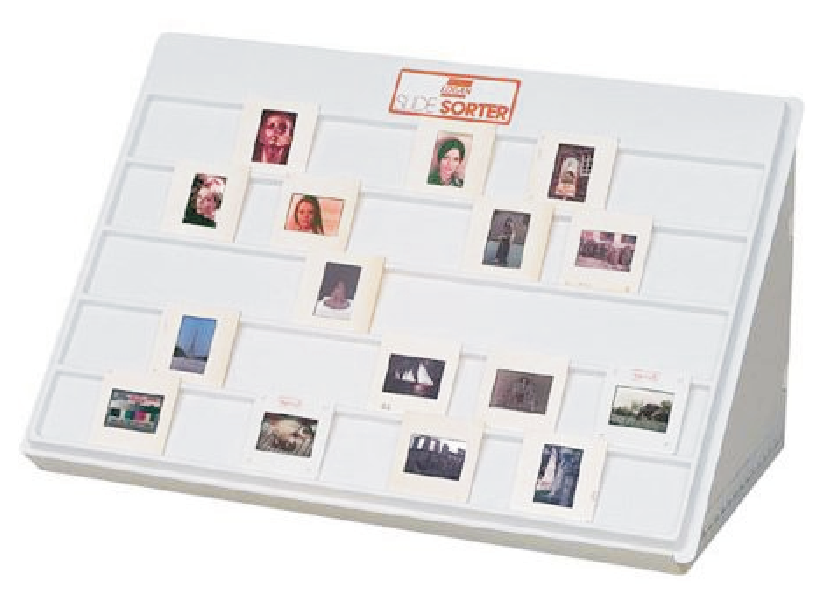
\includegraphics[width=0.5\linewidth]{planificacion/images/clasificadorAnalogico.eps} \\
  \caption{Ejemplo de clasificador de diapositivas anal�gicas}
  \label{fig:plan:clasificador}
  \end{center}
\end{figure}

El objetivo del clasificador anal�gico es que la persona sea capaz de organizar y clasificar las diapositivas de una manera r�pida y simple. La persona s�lo debe ir posicion�ndolas en las filas seg�n el orden que desee, e ir descartando las que no le satisfagan. Al finalizar la tarea tendr� las diapositivas situadas encima del clasificador en el orden deseado, y se tratar� simplemente de recogerlas y guardarlas en el mismo orden.

El objetivo de Apolo es imitar en la medida de lo posible el funcionamiento de estos clasificadores de diapositivas anal�gicos. Para ello Apolo ofrece las siguientes funciones:

\begin{enumerate}
\item Dentro de la aplicaci�n cada fotograf�a aparecer� mostrada como si de una diapositiva \emph{cl�sica} se tratara.
\item Cada diapositiva tiene un men� asociado, el cual ofrece la posibilidad de ver la imagen (a tama�o completo) o descartarla, as� como otros datos de inter�s que se consideren relevantes.% u observar los detalles de la misma (metadatos).
\item Para empezar a clasificar y ordenar fotograf�as es necesario primero haberlas importado a la aplicaci�n. Una vez importadas, % una carpeta o una serie de fotograf�as
	estas aparecer�n en la aplicaci�n como un conjunto de diapositivas
	esparcidas sobre una mesa. A esta zona la denominaremos precisamente \emph{Mesa}.
\item El usuario puede a partir de ese momento empezar a seleccionar las diapositivas que considere adecuadas y arrastrarlas a la \emph{zona de clasificaci�n o estanter�a}. En esta zona se simular�n una especie de baldas, similares a los de la Figura~\ref{fig:plan:clasificador}, donde se puedan depositar las diapositivas arrastradas.
\item El usuario puede en cualquier instante alterar el orden de las diapositivas en las estanter�as simplemente arrastrando la diapositiva hacia el lugar que desee.
\item Tambi�n puede cambiar la diapositiva de estanter�a de la misma forma, arrastr�ndola y solt�ndola en la estanter�a deseada.
\item Cada vez que el usuario haya conseguido ordenar de forma satisfactoria una secuencia de diapositivas, puede marcarla como subsecuencia ordenada y darle un nombre. A continuaci�n, todas las diapositivas se agrupar�n en un paquete, el cual tendr� una portada representativa de la subsecuencia; y se mover�n a una zona diferenciada que denominaremos de
	\emph{subsecuencias ordenadas o �lbum}. El aspecto de esta zona ser� como el de una estanter�a
    diferenciada, donde se disponen las subsecuencias horizontalmente.
\item El usuario tambi�n puede descartar todas las diapositivas que se encuentren en una estanter�a, dejando �stas de aparecer en la aplicaci�n.
\item En la zona de \emph{subsecuencias ordenadas o �lbum} se puede alterar el orden de las subsecuencias. Es decir, una subsecuencia reci�n a�adida, y que inicialmente se situar�a al final de la lista de subsecuencias, puede ser desplazada para colocarse entre dos subsecuencias ya existentes o al principio de la lista de subsecuencias.
\item Cuando en la zona superior de la aplicaci�n se encuentren todas las subsecuencias de diapositivas ordenadas de acuerdo a los deseos del usuario, �ste podr� exportarlas a un directorio o carpeta a su elecci�n. La aplicaci�n entonces crear� una copia de cada una de las fotograf�as seleccionadas en tal carpeta y las renombrar� de manera que preserven el orden deseado.
\item En ning�n caso se modificar�n o suprimir�n las fotograf�as originales (las que se importan). En cada exportaci�n se duplican tantas fotograf�as como sean necesarias.
\item Debe ser posible guardar el estado actual de la aplicaci�n en caso de que se tenga que interrumpir el proceso de clasificaci�n y se desee continuarlo m�s tarde.
\item El usuario, bas�ndose en estos estados parciales de la aplicaci�n, podr� crear �lbums de fotos de manera r�pida. Solo deber� abrir el fichero que contiene la clasificaci�n y orden de las diapositivas deseadas, y exportarlas a una determinada carpeta para obtener un conjunto de fotograf�as digitales en el orden deseado.
\end{enumerate}


%%==========================================================================================
%% NOTA(Pablo): P�rrafo de enlace.
%%==========================================================================================
Tras describir a grandes rasgos el funcionamiento de la aplicaci�n, la siguiente secci�n proporciona una visi�n de la metodolog�a que utilizaremos para su desarrollo, as� como las justificaciones para la elecci�n de la misma.

\section{Metodolog�a de Desarrollo}
\label{sec:planning:metodologia}

%%==========================================================================================
%% NOTA(Pablo): Frase de introducci�n.
%%==========================================================================================
Esta secci�n muestra detalladamente la metodolog�a de desarrollo que ser� utilizada durante la construcci�n de la aplicaci�n \emph{Apolo}.

La metodolog�a de desarrollo que se seguir� es la del \textbf{Modelo Iterativo Incremental}\cite{ite2002}. Se trata de un proceso de desarrollo evolutivo, en el cual la aplicaci�n se ir� construyendo mediante iteraciones, en cada una de las cuales, en base a incrementos, se otorgar�n m�s funcionalidades al sistema.
%Buscar una cita de alg�n personaje famoso

Esta metodolog�a requiere, inicialmente, una buena descripci�n del sistema o aplicaci�n a desarrollar. Es esencial que sea clara y lo m�s completa posible, pues a partir de ella se sustentar� todo el proceso de desarrollo.

\begin{figure}[!b]
  % Requires \usepackage{graphicx}
  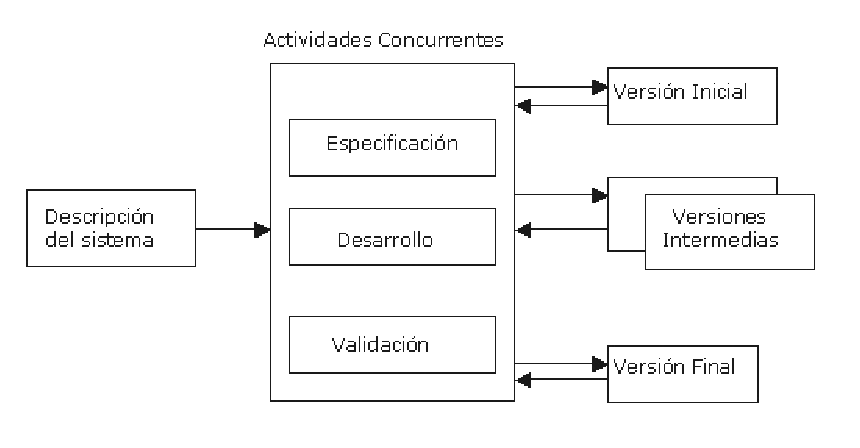
\includegraphics[width=\linewidth]{planificacion/images/mod-iterativo.eps}\\
  \caption{Modelo Incremental Iterativo}
  \label{fig:plan:modeloItera}
\end{figure}

Bas�ndose en la descripci�n se definen una serie de incrementos en donde cada uno a�ade m�s funcionalidades a la aplicaci�n, y por tanto cumple con una serie de requisitos. Debe comenzarse con la funcionalidad m�s b�sica de la aplicaci�n, de manera que pueda ir construy�ndose incrementalmente, es decir que cada versi�n incorpore a la anterior una funcionalidad nueva, la cual har� que se cumpla un requisito o varios.

Dentro de cada iteraci�n hay un proceso interno,
%que puede considerarse un ciclo de vida en Cascada
en el que pueden darse o no, las siguientes fases: an�lisis de los requisitos de esa iteraci�n, dise�o, implementaci�n y finalmente prueba del correcto funcionamiento. La primera iteraci�n dar� como resultado la versi�n inicial de la aplicaci�n con una funcionalidad muy b�sica, y solo cumpliendo los requisitos m�s b�sicos. A medida que vayan sucediendo iteraciones la aplicaci�n ira cobrando funcionalidad. En la �ltima iteraci�n se obtendr� el producto final, el cual debe cumplir todos y cada uno de los requisitos.

Las ventajas que tiene aplicar esta metodolog�a al desarrollo del proyecto Apolo es, que al ser la interfaz gr�fica una parte imprescindible al igual que la usabilidad, se puede en cada incremento ver si la soluci�n tomada es la adecuada para las expectativas esperadas, y en caso contrario corregirla antes de seguir avanzando en el desarrollo de la misma.

Adem�s gracias a que es un modelo evolutivo, se permiten (y es m�s, se esperan) cambios en los requisitos en tiempo de desarrollo. Lo cual permite cierto margen de cambio en el funcionamiento de la aplicaci�n.


\section{Requisitos de Alto Nivel de la Aplicaci�n}
\label{sec:planning:requisitos}

Esta secci�n muestra la identificaci�n de los requisitos de alto nivel que ha de satisfacer nuestra aplicaci�n software, de acuerdo a la descripci�n del �mbito funcional proporcionada en la Secci�n \ref{sec:plannning:ambito}.

Los requisitos de alto nivel encontrados son los descritos en el cuadro \ref{sec:planning:requisitos:tabla}.

\begin{table}[tb]
    \begin{center}
        \begin{tabular}{|c|p{9cm}|}
              \hline
              % after \\: \hline or \cline{col1-col2} \cline{col3-col4} ...
              Referencia & Requisito \\
              \hline  \hline
              R01 & Una fotograf�a deber� ser representada como una diapositiva. \\
              \hline
              R02 & La diapositiva podr� visualizarse o descartarse. \\
              \hline
              R03 & La aplicaci�n importar� las fotograf�as para trabajar con ellas. \\
              \hline
              R04 & Tras la importaci�n aparecer�n todas ellas en la zona baja de la aplicaci�n. \\
              \hline
              R05 & Las diapositivas deber�n poderse arrastrar hasta la zona media de la aplicaci�n donde habr� unas zonas donde depositarlas (baldas). \\
              \hline
              R06 & Una vez soltada la diapositiva en la zona central, deber� permanecer all� anclada. \\
              \hline
              R07 & Se podr�n recolocar las diapositivas dentro de cada estanter�a arrastr�ndolas. \\
              \hline
              R08 & Se podr� cambiar diapositivas entre estanter�as arrastr�ndolas. \\
              \hline
              R09 & Una balda, o subsecuencia de diapositivas, ya ordenada y clasificada, podr� ser almacenada en la zona superior de la aplicaci�n.  \\
              \hline
              R10 & Una balda, o subsecuencia de diapositivas, podr� ser descartada. \\
              \hline
              R11 & En la zona superior, se podr� reordenar subsecuencias de diapositivas. \\
              \hline
              R12 & Se podr� exportar la clasificaci�n y ordenaci�n a un directorio. \\
              \hline
              R13 & La exportaci�n deber� conservar el orden fijado durante el uso de la aplicaci�n. \\
              \hline
              R14 & No se modificar�n las fotograf�as originales, se copiar�n.  \\
              \hline
              R15 & Se podr� guardar el estado de la aplicaci�n en un fichero. \\
              \hline
              R16 & Se podr� cargar la aplicaci�n a un estado previo por medio de un fichero. \\
              \hline
        \end{tabular}
    \end{center}
    \caption{Requisitos de alto nivel}
    \label{sec:planning:requisitos:tabla}
\end{table}


\section{Iteraciones}
\label{sec:planning:Iteraciones}

En la siguiente secci�n se muestran las iteraciones planificadas a partir de la divisi�n de los requisitos de alto nivel encontrados, como puede verse en la secci�n \ref{sec:planning:requisitos}.

Las iteraciones planificadas de acuerdo a la agrupaci�n de funcionalidades son las siguientes:


\begin{enumerate}
	\item Importar fotograf�a, moverla (Drag \& Drop), visualizarla y descartarla. (Ver R01 y R02)
	\item Importar varias fotograf�as, llenar pool, realizar estanter�as. (Ver R03 y R04)
	\item Mover las diapositivas a la parte central y que se queden fijadas. (Ver R05 y R06)
	\item Recolocaci�n de diapositivas entre la misma estanter�a, cambio de diapositivas entre estanter�as. (Ver R07 y R08)
	\item Poder a�adir una balda a la zona superior, poder descartar balda. (Ver R09 y R10)
	\item Reordenar subsecuencias arrastr�ndolas entre la zona superior. (Ver R11)
	\item Exportar subsecuencias en el orden fijado. (Ver R12 y R13)
	\item Guardar el estado de la aplicaci�n. (Ver R15)
	\item Cargar la aplicaci�n al estado. (Ver R16)
	\item Retoques, Efectos visuales, correcci�n de bugs.
\end{enumerate}

Por cada iteraci�n pueden darse, si fueran necesarias cada una de las siguientes fases: an�lisis de los requisitos de esa iteraci�n, dise�o, implementaci�n y finalmente prueba del correcto funcionamiento.

Una vez descritas las iteraciones planteadas, en el siguiente cap�tulo se dise�aran los prototipos de los artefactos base del proyecto.

\section{Dise�o de los Artefactos Base del Proyecto}

En este cap�tulo se describen los artefactos b�sicos de los que constara el proyecto.
%%% Los artefactos comunes son:
%%  - La interfaz gr�fica
%%  - Haces un diagrama de clases con las estructuras de datos

Los artefactos b�sicos del proyecto Apolo son la interfaz gr�fica y la representaci�n de la fotograf�a como diapositiva dentro de la aplicaci�n. Son los elementos m�s b�sicos para el funcionamiento de la aplicaci�n.

La representaci�n de la fotograf�a como una diapositiva conlleva un dise�o de un componente que aparezca en la aplicaci�n simulando ser una diapositiva, para ello se ha esquematizado el dise�o del marco que tendr� que intentar evocar, lo m�ximo posible, el recuerdo de la diapositiva cl�sica. En la imagen \ref{fig:plan:esquemaMarcoDiapositiva} mostramos el dise�o planteado.


\begin{figure}[!tb]
 \begin{center}
  % Requires \usepackage{graphicx}
  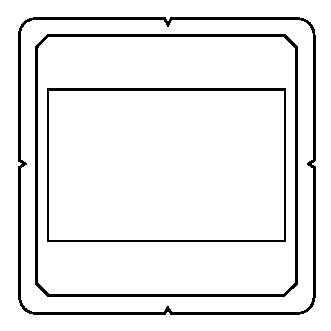
\includegraphics[width=0.3\linewidth]{planificacion/images/MarcoDiapositiva.eps}\\
  \caption{Esquema del Dise�o del Marco de la diapositiva.}
  \label{fig:plan:esquemaMarcoDiapositiva}
 \end{center}
\end{figure}

La interfaz gr�fica\cite{interfacesGUI} es un componente muy importante en el proyecto, pues se hace hincapi� en que debe ser atractiva y con una curva de aprendizaje muy corta y de pendiente muy suave. Para ello se pens� que la aplicaci�n constar�a de tres zonas claramente diferenciadas:

\begin{description}
	\item[Mesa] Se encuentra en la zona inferior de la aplicaci�n. En ella todas las fotograf�as importadas a la aplicaci�n y con las que se desea trabajar. Aparecer� una a continuaci�n de otra, de manera que el usuario sea capaz de seleccionar la que desee.
	\item[Zona de Clasificaci�n o Estanter�a] Esta en la zona central de la aplicaci�n, est� compuesta por baldas donde el usuario podr� ir \emph{posando} las diapositivas que vaya arrastrando, de manera que vaya ordenando y clasificando seg�n su gusto y criterio.
	\item[Zona de Subsecuencias Ordenadas o Album] Se ubica en la parte superior de la aplicaci�n, all� el usuario almacenar� las subsecuencias que considere ya ordenadas, de manera que cuando desee exportar, ser�n estas, seg�n el orden en el que se encuentren, las que ser�n exportadas.
\end{description}

La imagen de la Figura~\ref{fig:plan:esquemaDisenhoInterfaz} muestra un primer boceto de la interfaz gr�fica de la aplicaci�n, donde se pueden ver las diferentes zonas mencionadas en el listado anterior.


%***
% OK
%***
\begin{figure}[!tb]
  % Requires \usepackage{graphicx}
  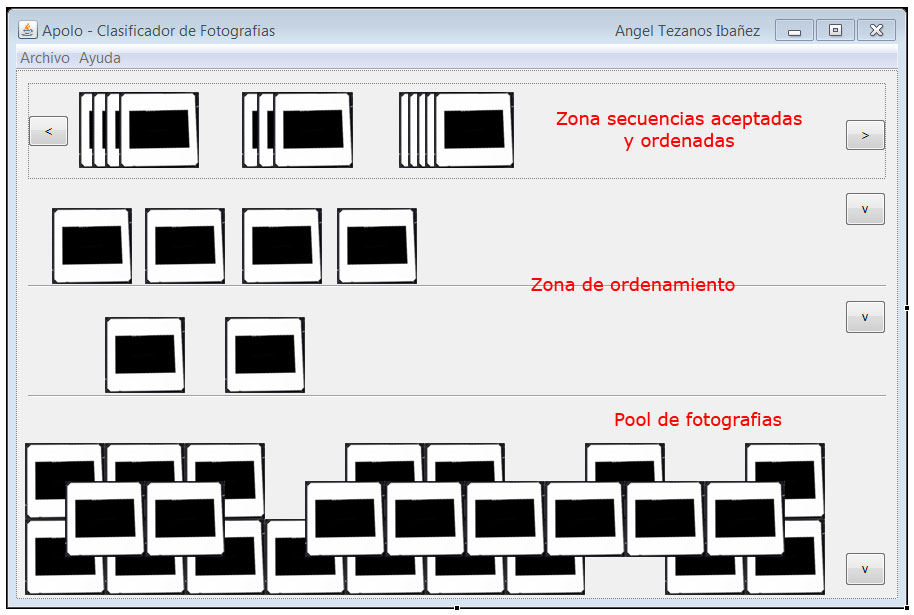
\includegraphics[width=\linewidth]{planificacion/images/MontajeInterfazGrafica.eps}\\
  \caption{Esquema del Dise�o Inicial de la Interfaz Gr�fica.}
  \label{fig:plan:esquemaDisenhoInterfaz}
\end{figure}

%*=============
% Igual explicarlo un poco mejor
%*=============

\begin{figure}[!htb]
  % Requires \usepackage{graphicx}
  \begin{center}
    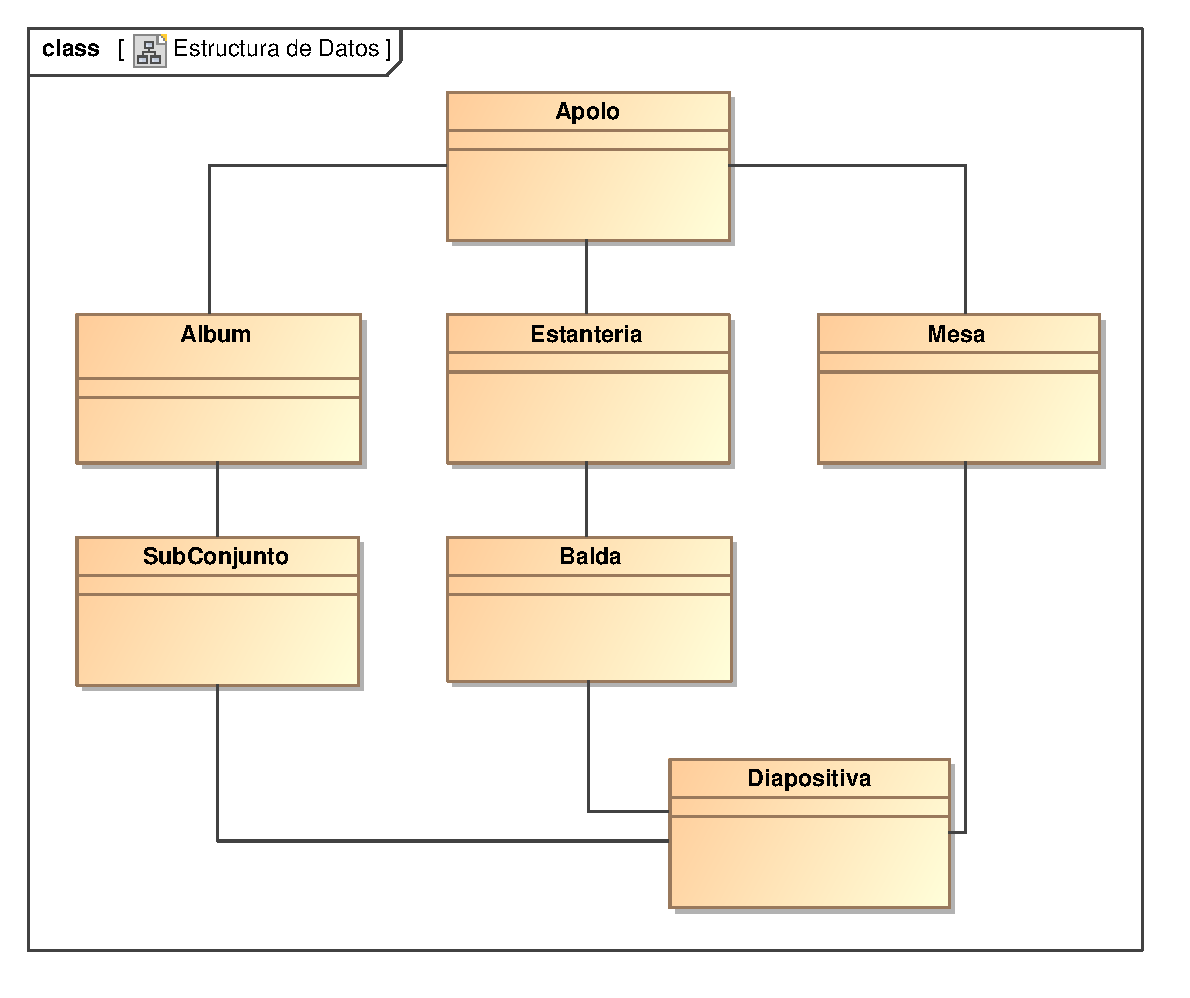
\includegraphics[width=0.8\linewidth]{planificacion/images/EstructuraDeDatos.eps}
  \end{center}
  \caption{Esquema del Dise�o de la estructura de datos.}
  \label{fig:plan:esquemaDisenhoEstrucDatos}
\end{figure}


Para completar el dise�o de los artefactos que componen la aplicaci�n, se realiz� a muy alto nivel la estructura de datos que tendr� \emph{Apolo}. Puede verse en la figura \ref{fig:plan:esquemaDisenhoEstrucDatos} como se relacionan los componentes de la aplicaci�n.

Una vez descritos los artefactos base de los que constar� la aplicaci�n, en el siguiente cap�tulo se hablar� sobre las herramientas usadas para la implementaci�n de los mismos.


\section{Herramientas utilizadas para el desarrollo de la aplicaci�n}

En esta secci�n se describen las herramientas utilizadas para la creaci�n de la aplicaci�n.

Para el dise�o UML\footnote{Unified Modeling Language}\cite{uml} se ha utilizado la herramienta Magic Draw
La implementaci�n de la aplicaci�n se desarroll� con ayuda del entorno de desarrollo Eclipse\cite{eclipse}, junto con unos plugins para la creaci�n de interfaces visuales y el control de versiones.

Como repositorio donde almacenar las distintas versiones, se utiliz� el servicio ofrecido por google code.

El sistema operativo donde se desarrollar� ser� a parte igual en un sistema \emph{Microsoft Windows 7}\cite{win7} y \emph{Ubuntu 10.10}\cite{ubun}.



\section{Construcci�n de Prototipos}

En esta secci�n se detalla la construcci�n de un primer prototipo de diapositiva, donde se investigar� que soluci�n tomar para representar mejor el movimiento de \emph{Drag and Drop}.

%%  Hacer una bean diapositiva, cargar una diapositiva y moverla
El prototipo construido es una aplicaci�n simple en la que aparece una diapositiva y esta puede ser arrastrada por la aplicaci�n. Al arrastrarla entra en acci�n un efecto de \emph{Drag And Drop} el cual consiste en el la aparici�n del componente (en este caso la diapositiva) que se arrastra de forma transl�cida siguiendo el movimiento del rat�n, de esta manera ayuda al usuario a localizar con exactitud donde se arrastra la diapositiva y cu�l de todas est� arrastrando. Esto puede verse en la figura \ref{fig:plan:DnD}, este prototipo servir� para investigar y conocer la t�cnica del \emph{Drag and Drop} algo fundamental en el uso de la aplicaci�n si queremos que su uso resulte f�cil y atractivo.


\begin{center}
	\begin{figure}
		 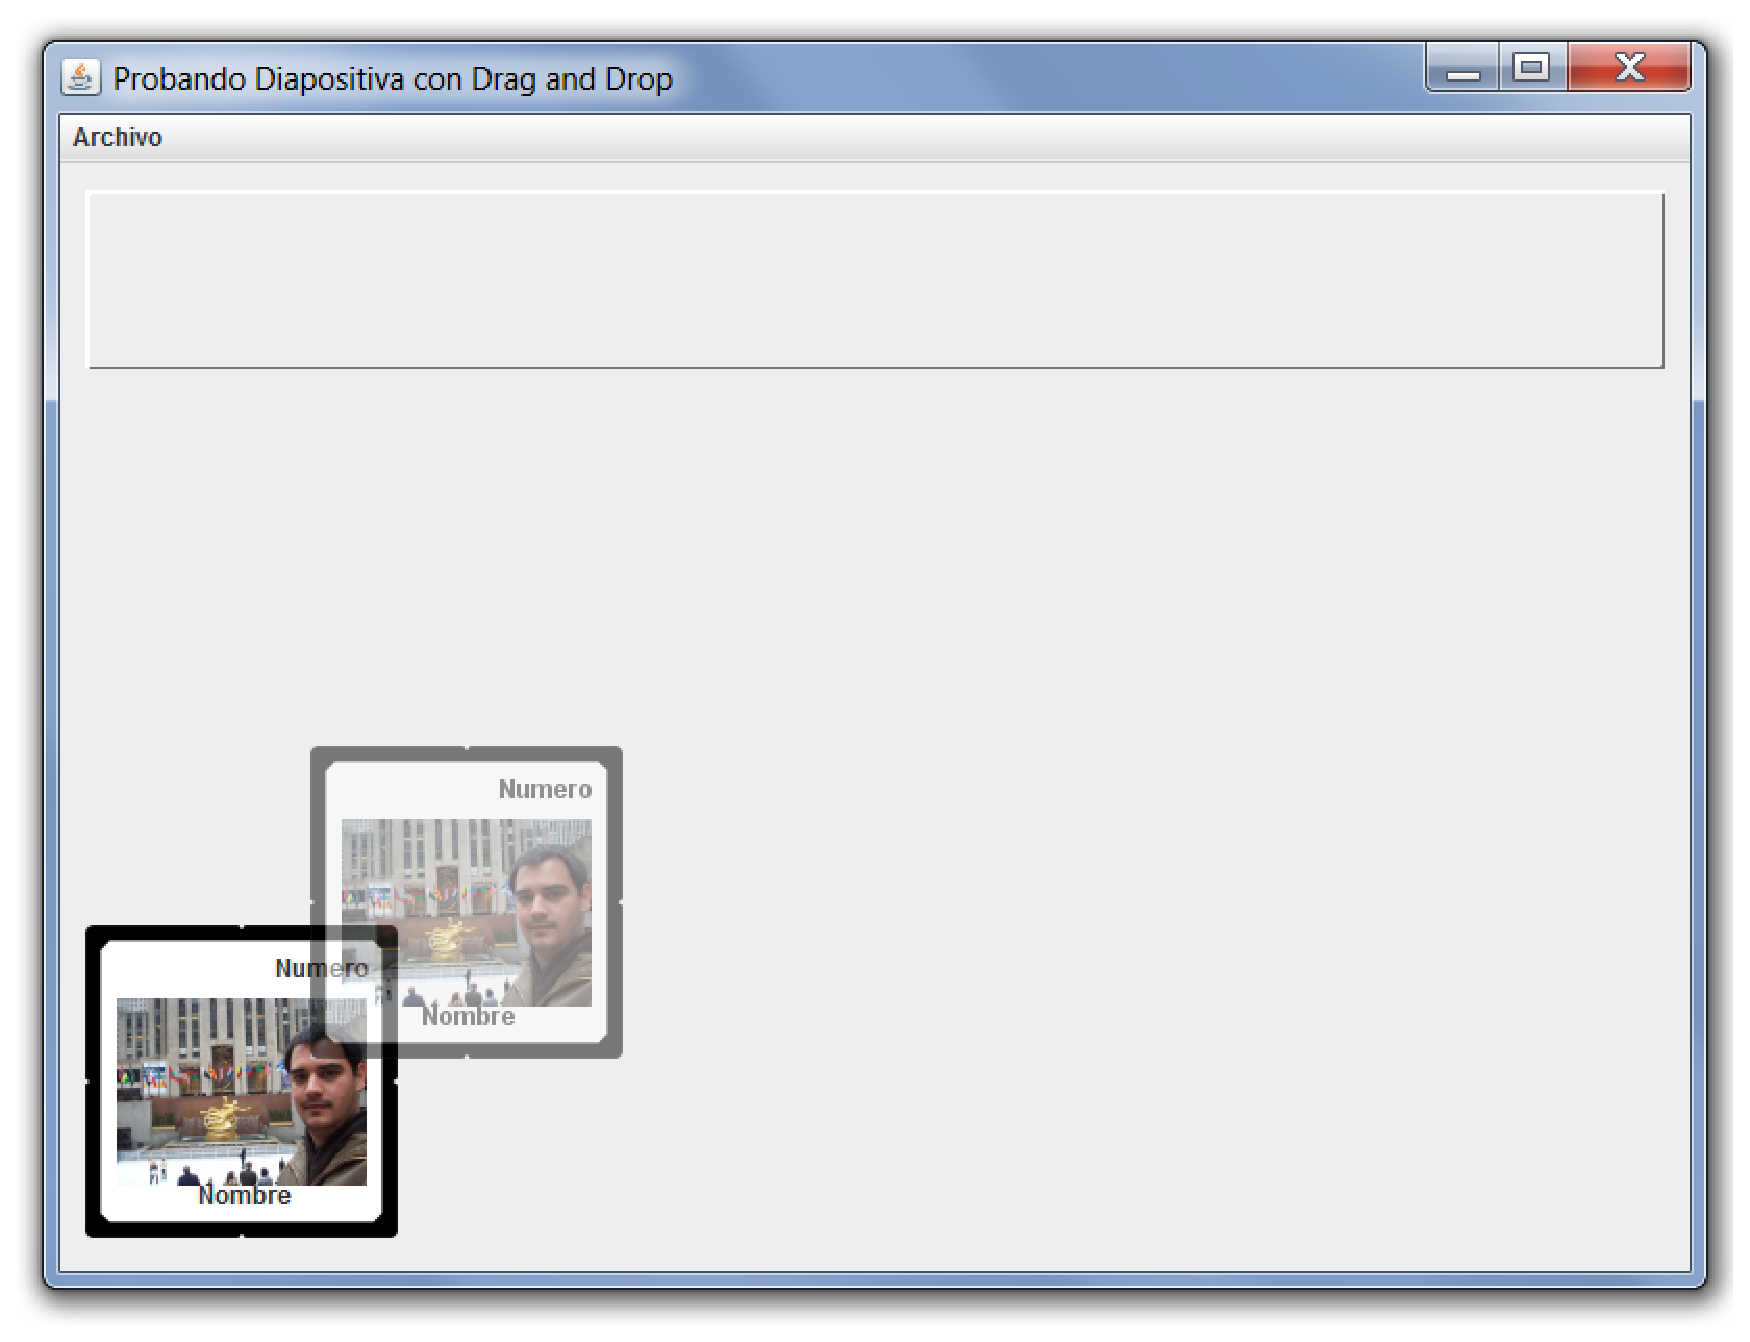
\includegraphics[width=\linewidth]{planificacion/images/prototipo.eps}
		\caption{Efecto de Drag and Drop}
		\label{fig:plan:DnD}
	\end{figure}
\end{center}

\section{Sumario}

Durante este cap�tulo se ha descrito la planificaci�n del proyecto fin de carrera, indicando el �mbito funcional en el que se encuentra, as� como la metodolog�a que se usar�. Tambi�n se describieron los requisitos de alto nivel y las distintas iteraciones de las que se compondr� el proceso de desarrollo.

Tambi�n se describi� el dise�o de los componentes m�s b�sicos del proyecto as� como las herramientas que se utilizaran para llevarlo a cabo. Finalmente se mostr� la construcci�n del prototipo con el que se ensayaran pruebas del \emph{Drag and Drop}. 

% Cap�tulo 3: Antecedentes
%=============================================================================%
% Author : Angel Tezanos Iba�ez                                               %
% Author : Pablo S�nchez Barreiro                                             %
% Version: 2.0, 23/02/2011                                                    %
% Master Thesis: Introduction                                                 %
%=============================================================================%

\chapterheader{Antecedentes}{Antecedentes}
\label{chap:introduction}

El presente cap�tulo describe brevemente las tecnolog�as sobre las que se fundamenta el presente proyecto. M�s concretamente, se explica el funcionamiento del software basado en componentes, en especial Java Beans.

\chaptertoc

\section{Desarrollo de Software basado en Componentes}

El proyecto se desarrollara bajo una programaci�n orientada a componentes. Esta rama de la ingenier�a software trata de construir sistemas a base de componentes funcionales, como si de un lego se tratase. Para ello cada componente debe tener una interfaz bien definida.

El nivel de abstracci�n de de los componentes se considera mas alto que el de los objetos al agrupar unidades funcionales autonomamente. De esta manera se explota en gran medida las posibilidades de reutilizaci�n. Pudiendo utilizar componentes ya creados por otros, y/o en otros proyectos de manera r�pida y sencilla.

Cada componente software es un elemento o pieza del sistema final que ofrece un servicio y es capaz de comunicarse con el resto de componentes. b�sicamente un componente es un objeto escrito siguiendo unas especificaciones, si las cumple adquiere la caracter�stica de \textbf{reusabilidad}.

Los componentes deben poder ser serializados para garantizar el envi� del estado del objeto a trav�s de flujos de datos.

Para que un componente este bien dise�ado requiere un esfuerzo en la fase de dise�o, pues se debe tener en cuenta que puede ser reutilizado por muchos programas, debe estar debidamente documentado, probado de manera enf�tica, es decir, se debe probar la validez de las entradas y que sea capaz de mostrar mensajes de error claros y oportunos; tambi�n se debe prever el uso del componente de manera imprevista o incorrecta.

\section{Java beans como modelo de componentes}

JavaBeans es la tecnolog�a de componentes de Java, cada componente se le conoce como bean, como se dijo anteriormente, un bean no es mas que una clase de objetos con unas caracter�sticas especiales:

\begin{enumerate}
	\item Es una clase publica que implementa la interfaz serializable
	\item Expone una serie de propiedades que pueden ser le�das y modificadas por el entorno de desarrollo.
	\item Los eventos que posea pueden ser capturados y asociados a una serie de acciones.
\end{enumerate}

% Sin n�mero \begin{itemize}

Las propiedades no son mas que atributos del objeto que pueden ser modificados y le�dos por el entorno de desarrollo. Cada propiedad debe tener al menos un m�todo get para obtener el valor, y un set para modificarlo. En caso de que no se implemente el m�todo set se entender� que es una propiedad de solo lectura.

Existen varios tipos de propiedades:
\begin{itemize}
    \item Simples: Representa un �nico valor
    \item Indexadas: Representa un array de valores
    \item Ligadas (Bound): Notifican un cambio de la propiedad a otros objetos (listeners).
    \item Restringidas (Constrained): Similar a la Ligada salvo que los objetos notificados tienen la opci�n de vetar el cambio.
\end{itemize}

%%Extender mas si es posible 
Gracias a esta tecnolog�a podemos dise�ar componentes que iremos a�adiendo a nuestra aplicaci�n de manera que incremental. Es decir, nos centraremos en la creaci�n de un componente, y cuando este este implementado, procederemos al siguiente, de manera que el trabajo de dise�o e implementaci�n este repartido en fases. 


% Cap�tulo 5: Ingenier�a de Requisitos

% Cap�tulo 6: Definici�n Arquitect�nica y Dise�o Software

% Cap�tulo 7: Construcci�n e Implementaci�n

% Cap�tulo 8: Pruebas

% Cap�tulo 9: Despliegue y Aceptaci�n

% Cap�tulo 10: Discusi�n, Conclusiones y Trabajos Futuros

% CONTENT: Appendices, if desired
\renewcommand\chaptername{Appendix}                      % hereafter, chapters are called "Appendix"
\renewcommand\thechapter{\Alph{chapter}}        % chapter number in Romans
\renewcommand\thesection{\Alph{chapter}.\alph{section}}  % make sections "I.a", instead of "1.1"
\setcounter{chapter}{0}                                  % start numbering chapters from 1 on again


% Appendix A:
% \appendix

\chapter{Contenidos del CD}

En este capitulo se muestra el contenido del CD adjunto a esta memoria, el cual aporta contenido multimedia as� como instal�ndose y c�digo fuente.
\newline

El CD contiene los siguientes elementos:
\begin{itemize}
    \item {\bfseries C�digo Fuente:} C�digo Fuente de la aplicaci�n desarrollada.
    \item {\bfseries Instaladores:} Instaladores de la aplicaci�n para los distintos Sistemas Operativos.
    \item {\bfseries Manual de usuario:} Manual de usuario de la aplicaci�n.
    \item {\bfseries Memoria del proyecto:} Memoria del proyecto en formato \emph{pdf}.
    \item {\bfseries VideoTutoriales:} Videotutoriales con las acciones mas comunes de la aplicaci�n.
    \item {\bfseries Web:} P�gina Web de la aplicaci�n.
\end{itemize} % Appendix I

% CONFIG: Bibliography style
% \cleardoublepage                            % start in right side page
\addcontentsline{toc}{chapter}{References}  % add this "chapter" to the ToC, with the name "Bibliography"
%\bibliographystyle{alpha}                  % bibliography style
\bibliographystyle{abbrv}                  % bibliography style
% \bibliography{references/references}

\end{document}
